\section{Consistency Tests}

Here I collect together a number of internal and external consistency
checks to verify correctness of the code and performance.

\subsection{Side-by-side Comparison of \betamodel\ fitting with \markov}

As a sanity check, Stephen and I ran a comparison of \climax\ and
\markov\, fitting an asymmetric \betamodel\ to SZA data for Abell1914.
Results are in Figure~\ref{fig:fig1}.  The resulting chains give
nearly identical results for all parameters (except that
\markov\ prefers a slight shift ($\sim 5$ arcsec) in the x-centroid
for some reason that I have not investigated; I believe this
corresponds roughly to the image pixelation in \markov\ and I suspect
that the model centroid is erroneously shifted by 1 pixel).  The
\climax\ chain is significantly longer, since it took two orders of
magnitude less time to run.

\newpage
\begin{figure}[mh]
\begin{center}
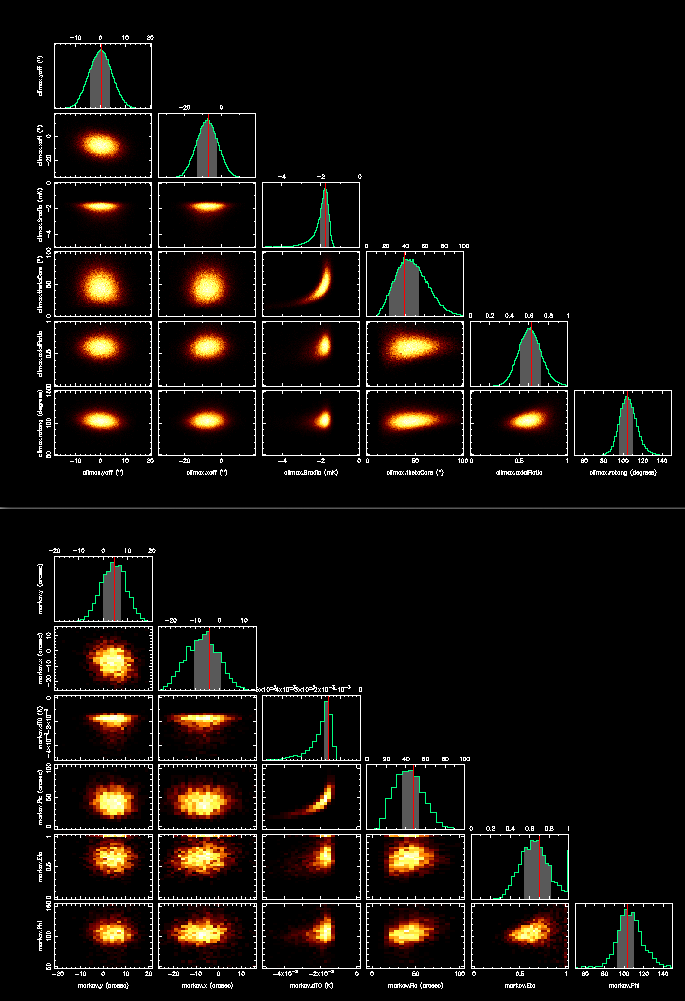
\includegraphics[scale=0.45]{figures/climax_markov_comp.png}
\end{center}
\caption{Top panel: \climax\ \betamodel\ run for A1914.  Bottom panel:
  \betamodel\ run in \markov\ (for the same priors).  Parameters are
  shown in the same order and to the same scale (note, however, that the
  \climax\ chain is significantly longer, hence the smoother distributions).}
\label{fig:fig1}
\end{figure}

\newpage
\subsection{Sanity check on 3D radial-profile fitting}

The \betamodel\ is defined as the 2D shape function

\begin{equation}
f(x) = {1\over{\left[1 + x^2\right]^{(1-3\beta/2)}}},
\end{equation}

frequently used to fit $y(\theta) = y(0)f(\theta)$, for example.

As a cross-check on \climax\ fitting using integrated 3D radial
profiles, I can reconstruct the 2D beta model by starting the 3D
radial profile (i.e., for an isothermal model $T(r) = T_0$ this would
be a density model)

\begin{equation}
p(x) = {1\over{\left[1 + x^2\right]^{3\beta/2}}}
\end{equation}

and performing the line integral to recover the 2D beta model shape.

Finally, I can use the GNFW model itself

\begin{equation}
p(x) = {1\over{x^\gamma\left[1 + x^\alpha\right]^{(\epsilon-\gamma)/\alpha}}}
\end{equation}

which reduces to the \betamodel\ profile for $(\alpha,\epsilon,\gamma)
= (2, 3\beta, 0)$.  Then the identical code that generates the Arnaud
and other variants of the GNFW models can be used to generate the
integrated \betamodel\ as well.

The integrated profiles constructed in these last two ways match the
analytic 2D \betamodel\ profiles to better than a part in $10^{-5}$, and
parameters derived from fitting either model show good agreement (see
Figure~\ref{fig:fig2}).  There are some small differences, however,
notably a longer tail in $\theta_c$ for the \betamodel\ that is less
pronounced in the integrated versions.

\newpage
\begin{figure}[th]
\begin{center}
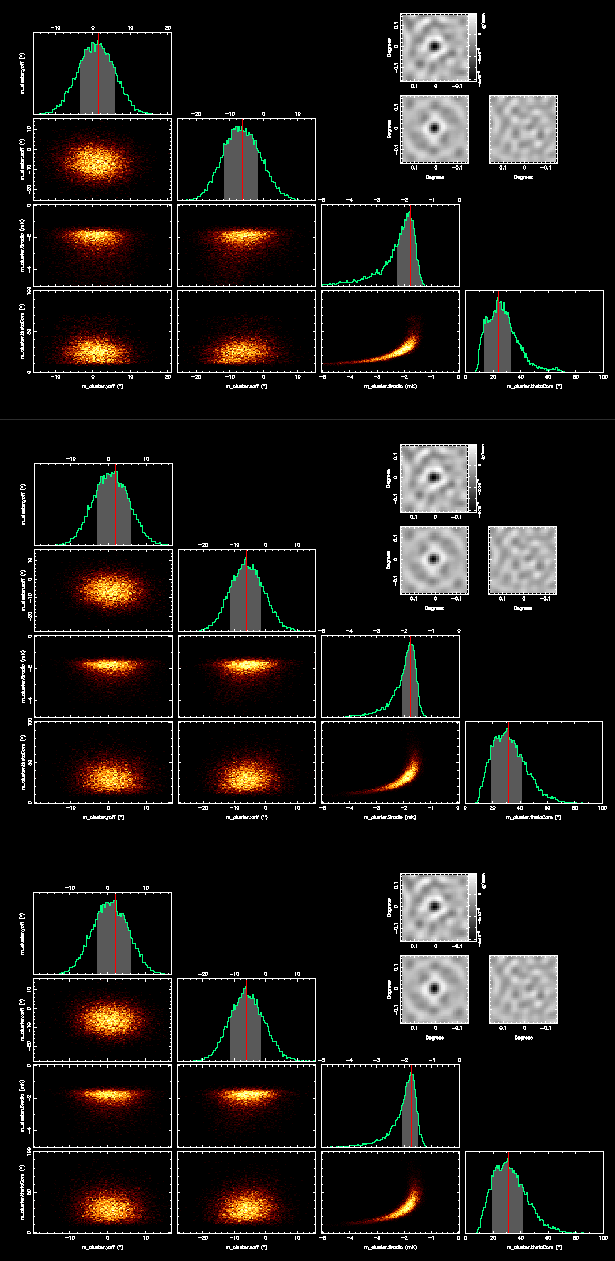
\includegraphics[scale=0.35]{figures/beta_model_comps.png}
\end{center}
\caption{Top panel: \climax\ 2D \betamodel\ fits for A1914.  Middle
  panel: integrated \betamodel\ fit in \climax\ using the 3D (i.e.,
  density) profile.  Bottom: Integrated \betamodel\ fit using the same
  GNFW profile code that generates the Arnaud model, etc. (with a
  generalization of the GNFW profile that allows it to reduce to the
  \betamodel\ profile for suitable choice of parameters). Images in
  the top right are, counter-clockwise from top left, dirty map of
  data, dirty map of model, residuals.}
\label{fig:fig2}
\end{figure}

\newpage
\subsection{Side-by-side comparison of \nagaimodel\ fitting with \markov}

Originally I was concerned that physical parameters I derived from my
\arnaudmodel\ fits to A1914 didn't match the parameters given in
Tony's paper (or even gave me ballpark numbers for A1914's total mass,
see \S\ref{sec:confusion}).  This turns out to be an artifact of the
particular data set I have been using for testing.  Fits to the two
datasets do indeed give fairly different results for $\theta_c$ but a
direct comparison of fitting the \nagaimodel\ to the same dataset in
\climax\ and \markov\ shows good agreement (see
Figure~\ref{fig:nagaicomp}).  

Moreover, using the \nagaimodel\ normalization, I determine

\begin{eqnarray}\nonumber
\R500  &=& 1.2\pm0.3~{\rm Mpc}\\\nonumber
\Mt500 &=& 4.2\pm2.5\times 10^{15}~\Msolar
\end{eqnarray}

where the $\R500$ and $\Mt500$ constraints comes directly from the
\nagaimodel\ fits.

This is to be compared with $\R500 = 1.3\pm0.1~{\rm Mpc}$ from
Tony's N07 fits, and $\Mt500 = 2-3\times 10^{15}~\Msolar$ I've seen in
the literature.  

By comparison, the \arnaudmodel\ fits I described in
\ref{sec:confusion} yield $\R500 = 0.43~{\rm Mpc}$ and $\Mt500 =
8\times 10^{15}~\Msolar$.  But those fits were not to the same dataset
used in this analysis.  I therefore conclude that the 3D radial
profile-fitting in \climax\ is consistent with the fitting in
\markov\ and that the discrepancy between the results derived here and
the results described in \S~\ref{sec:confusion} do not indicate any
problem with the fitting code, but rather one of three things:

\begin{list}{}{\labelwidth 0.4in \leftmargin \labelwidth \addtolength{\leftmargin}{\labelsep}}

\item[1] {a problem with that data set}

\item[2] {a disagreement between the \nagaimodel\ normalization and the
  \arnaudmodel\ normalization}

\item[3] {they indicate that there are large systematic errors that
  are not showing up in the formal errors from the Markov chains. For
  instance, the likelihood for the GNFW model parameter space may be
  multimoded, implying that very different combinations of ${P_e}_0$
  and $\theta_c$ can provide a good fit to the outer cluster profile
  and therefore to the SZ data, even though they imply very different
  physical results.}
\end{list}

At this point, I think the first possibility is likely, since a
\nagaimodel\ fit to that data give a similar normalization to the data
fit in this section, but a $\theta_c$ that is smaller by nearly $60\%$
(hence implying a larger pressure for the same
$y$ normalization and therfore a larger mass).

\newpage
\begin{figure}[th]
\begin{center}
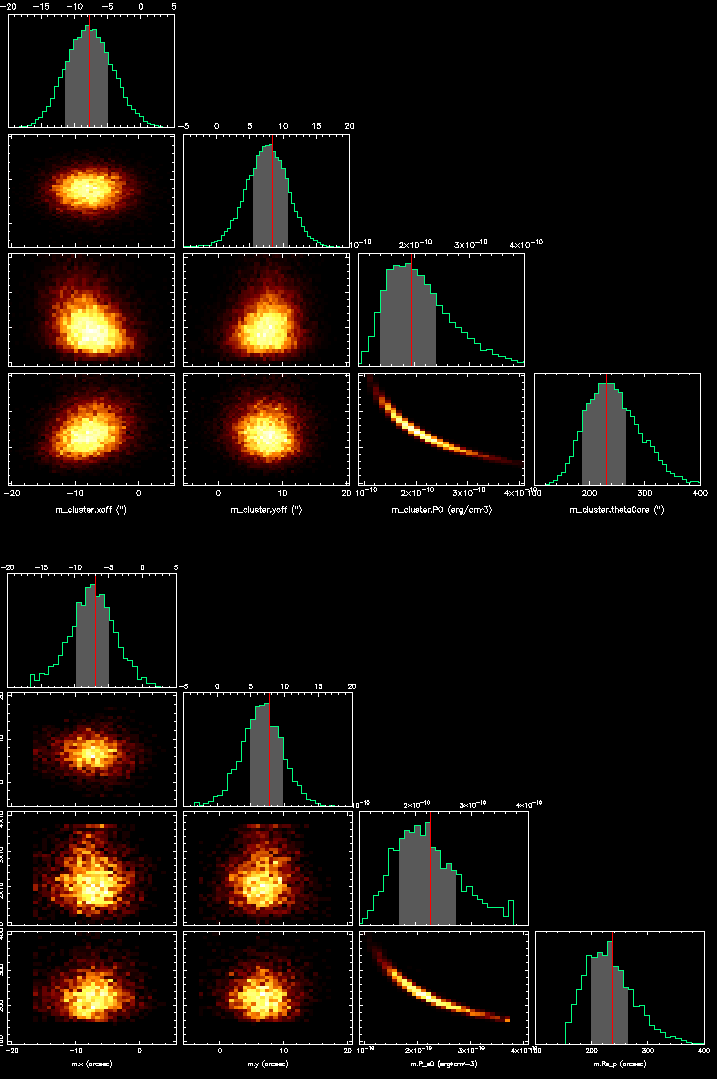
\includegraphics[scale=0.4]{figures/climax_markov_nagai_comp.png}
\end{center}
\caption{Top panel: \climax\ 2D \nagaimodel\ fits for A1914 (NB: this
  is to the same dataset that Tony used for his profile paper, which
  gives significantly different results at least for $\theta_c$ to the
  dataset I used for the \betamodel\ comparison).  Bottom:
  \nagaimodel\ fit in \markov.  Third colum in the \climax\ plot is
  the pressure derived from the temperature normalization fit to the
  data, in units of ${\rm erg/cm^3}$, to compare to the ${P_{e}}_0$ output by \markov.}
\label{fig:nagaicomp}
\end{figure}
